%!TEX root = dippa.tex
%%% This file contains the MicroRNAs section of my master's thesis.
%%% This section covers the biological background of miRNAs.
%%% Author: Viljami Aittomäki

\section{MicroRNAs}\label{micrornas}

MicroRNAs (miRNAs) are a class of endogenous (i.e. synthesized within the
cell) non-coding small RNA molecules that function as post-transcriptional
regulators of gene expression \citep{Ambros2004}. In their
functional, mature form miRNAs are single stranded and approximately 22
nucleotides long. MicroRNAs are not translated into protein. Instead, they
have an important role in regulation of gene expression in a wide range of
physiological, developmental and pathological processes \citep{Bartel2009}.
MicroRNAs assert their regulatory function by destabilization and degradation
of target messenger RNA (mRNA) molecules and inhibition of mRNA translation
\citep{Fabian2010}.




\subsection{Discovery of microRNAs}

The first known microRNA, lin-4, was discovered in 1993 by two research groups
studying the larval development of the nematode \emph{Caenorhabditis elegans}.
The researchers noted that lin-4 does not encode a protein, but instead
produces a pair of small RNAs, the longer of which was proposed to be a
precursor to the shorter one \citep{Lee1993}. The RNAs encoded by lin-4 were
noted to have conserved antisense complementarity in several sites of an
untranslated region of the lin-14 mRNA, and these sites were found to be
necessary for the normal repression of lin-14 expression by lin-4
\citep{Lee1993,Wightman1993}.
%It
%should be noted, that one of these groups also showed that lin-4 reduces the
%amount of the LIN-14 protein -- the end-product of the lin-14 gene -- without
%significantly affecting the cellular concentration of the lin-14 mRNA
%\citep{??}. %oks tää Wightman1993:ssa?
%We will return to the issue of microRNA action in chapter \ref{microrna-function}.

Let-7, the second microRNA to be discovered, was also first found in \emph{C.
elegans}, however, homologues of let-7 were later found in several other
species \citep{Pasquinelli2000}. Soon after, numerous microRNA genes were found across
a variety of species, and a registry was set up to serve as a comprehensive
knowledge base of published microRNAs and as an independent authority on
microRNA nomenclature \citep{GriffithsJones2004}. This registry later became
miRBase, the de facto reference database of known microRNAs, and now provides
sequence data, annotations, as well as links to databases of predicted and
validated target genes for miRNAs \citep{Kozomara2014}.




\subsection{MicroRNA genomics}\label{microrna-genomics}

The number of known small RNAs has since vastly expanded and microRNAs have
been found in more than 200 organisms, including all studied animals, plants
\citep{JonesRhoades2006} and viruses \citep{Grundhoff2011}. The number of
records in miRBase has risen exponentially
% from 218 mature miRNAs in the first release in 2002
to 35,828 mature miRNAs for 223 species (including 2,588 human miRNAs) in the
most recent version (v21, released June 2014 \citep{MiRBaseWeb}). This
illustrates the large number of novel microRNA molecules discovered recently,
which has been mainly due to increasing efforts in and availability of
sequencing. miRBase lists 2,588 known human miRNAs at the time of writing this
thesis.
% A web service called
% miRBaseTracker has been developed by \citet{VanPeer2014} for updating miRNA
% nomenclature and annotations across different versions of miRBase.
% to allow correct comparison of miRNA study results and reannotation
% of miRNA analysis platforms.

MicroRNAs are highly conserved in evolution \citep{Bartel2004}. For instance,
approximately 55\% of \emph{C. elegans} miRNAs have homologues in humans
\citep{IbanezVentoso2008}. Interestingly, the
appearance of multi-cellular organisms appears to co-occur with the appearance
of the microRNA machinery. Organism complexity and speciation also seem to
correlate with miRNA complexity, together suggesting that microRNAs have had a
crucial role in the development of complex organisms \citep{Lee2007}.

MicroRNAs are found in varying genomic contexts in the DNA. Approximately 50\% of
mammalian miRNAs are located in close proximity to other miRNAs and form
polycistronic miRNA clusters that are transcribed simultaneously. Some miRNAs
reside in the genome as dedicated miRNA genes, with their own promotor regions.
\citep{Kim2009} miRNAs and miRNA clusters can be situated in exons or
introns of non-coding genes and some are found in introns of protein-coding genes
\citep{Du2005}.
% MicroRNAs located in introns are referred to as
% mirtrons \citep{Ruby2007}.

MicroRNAs are expressed in all tissues, however, different tissues have
differing miRNA expression profiles \citep{Krol2010}. Many microRNAs also have
differing expression in different developmental stages of an organism, often
functioning as molecularer switches to move between stages. For instance,
let-7 functions to control the transition from late larval to adult stage in
\emph{C. elegans} \citep{Bartel2004}.

% Tight evolutionary control, extensive transcriptome
% targeting, and the fact that miRNAs and their associated proteins are one of
% the most abundant molecules in the cytoplasm \citep{Bartel2004} highlight the
% importance of microRNAs.




\subsection{MicroRNA biogenesis}\label{microrna-biogenesis}

The canonical pathway of microRNA biogenesis is illustrated in Figure
\ref{fig:mirna-biogenesis} and is presented here as reviewed by \citet{Bartel2004},
\citet{Melo2011}, \citet{Ha2014}, and many others. 

Most microRNAs are transcribed from genomic DNA by RNA polymerase II to form a
long primary microRNA (pri-miRNA) molecule \citep{Lee2004}. The pri-miRNA molecule
contains a hairpin structure, with a 33-bp double-helix stem and a terminal
loop, and flanking single-strand sequences, which are several hundreds or
thousands of nucleotides long \citep{Kim2005}. Some miRNAs within Alu repeat elements
can be transcribed by RNA polymerase III \citep{Borchert2006}.

The pri-miRNA is cut by the ribonuclease Drosha to form
%one or, in the case of polycistronic miRNAs, several
a pre-microRNA (pre-miRNA), which consists of the hairpin and is approximately
70 nt long \citep{Lee2003}. Examples of typical pre-miRNA structure are shown in Figure
\ref{fig:premirna-structure}. Drosha is aided by the essential cofactor DGRC8
%(the protein product of a gene deleted in DiGeorge syndrome \citep{Shiohama2003})
and they form a complex known as the Microprocessor \citep{Gregory2004}.
The hairpin is then exported from the nucleus to the cytoplasm by Exportin 5
(XPO5), a member of the nuclear transport receptor family \citep{Lund2004}.

\begin{figure}[htb]
  \centering
  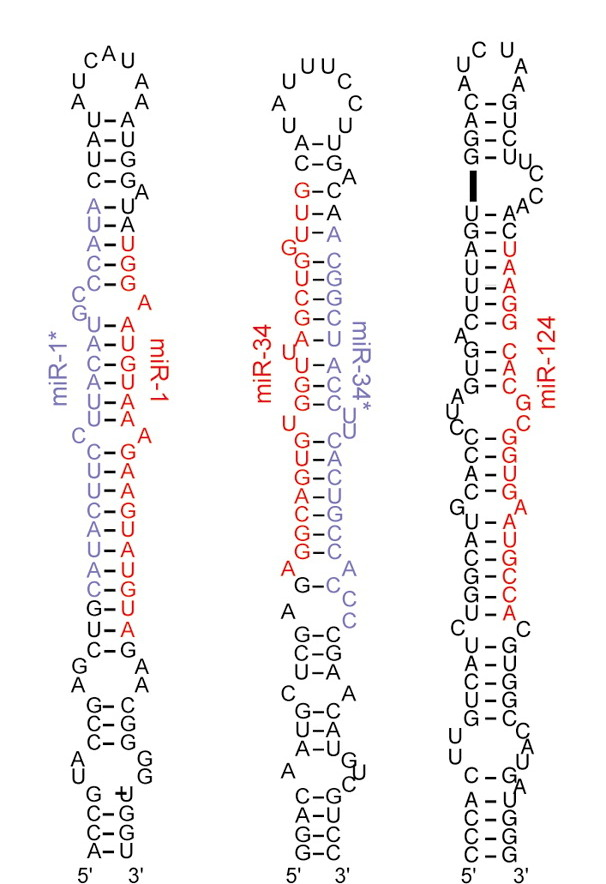
\includegraphics[width=0.4\linewidth]{figures/premiRNA_structure.png}
  \caption{Hairpin structure of three pre-miRNAs from \emph{C. elegans}.
  Red and gray colors indicate the sequences of mature miRNAs.
  Reprinted with permission from \citep{Bartel2004}.}
  \label{fig:premirna-structure}
\end{figure}

In the cytoplasm, the ribonuclease Dicer cleaves out the loop of the hairpin
to form a 22-nt-long double-stranded miRNA:miRNA* duplex corresponding to
the stem of the hairpin \citep{Bernstein2001}.
Dicer associates with a cofactor, in humans TRBP (Tar RNA-binding protein),
which is not required for effective dicing of the pre-miRNA,
but acts to physically bridge the Dicer to an Argonaute protein
% for further miRNA processing
\citep{Chendrimada2005}.

The duplex is then bound by the Argonaute protein, in mammals one of Ago1
through Ago4, forming what is called the RNA-induced silencing complex (RISC).
The RISC is a protein complex containing Dicer, TRBP and Ago \citep{Gregory2005}.
Ago, aided by Dicer and TRBP, unwinds the strands of the duplex and retains one of
them. The retained strand is known as the guide strand (or miRNA). The other
strand, called the passenger (or miRNA*), is released and typically degraded \citep{Du2005}.
In some instances, either one of the strands can become the guide
or both can be used \citep{Czech2009}.
%Notably, the Dicer cleaving, duplex unwinding and eventual
%mRNA regulation activity are, in fact, all coupled and performed by RISC
%\citep{Gregory2005}.

Not all miRNAs are generated through this canonical pathway of microRNA
biogenesis. Some miRNAs are not dependent on Drosha, such as mirtrons, which
are cut into pre-miRNA by the spliceosome, a molecular complex responsible for
removing introns (and sometimes exons) from precursor mRNA \citep{Ruby2007}. The
biogenesis of miR-451 is independent of Dicer; miR-451, which
has an important role in erythropoiesis, is cleaved by Ago2 \citep{Cheloufi2010}.

\begin{figure}[htb]
  \centering
  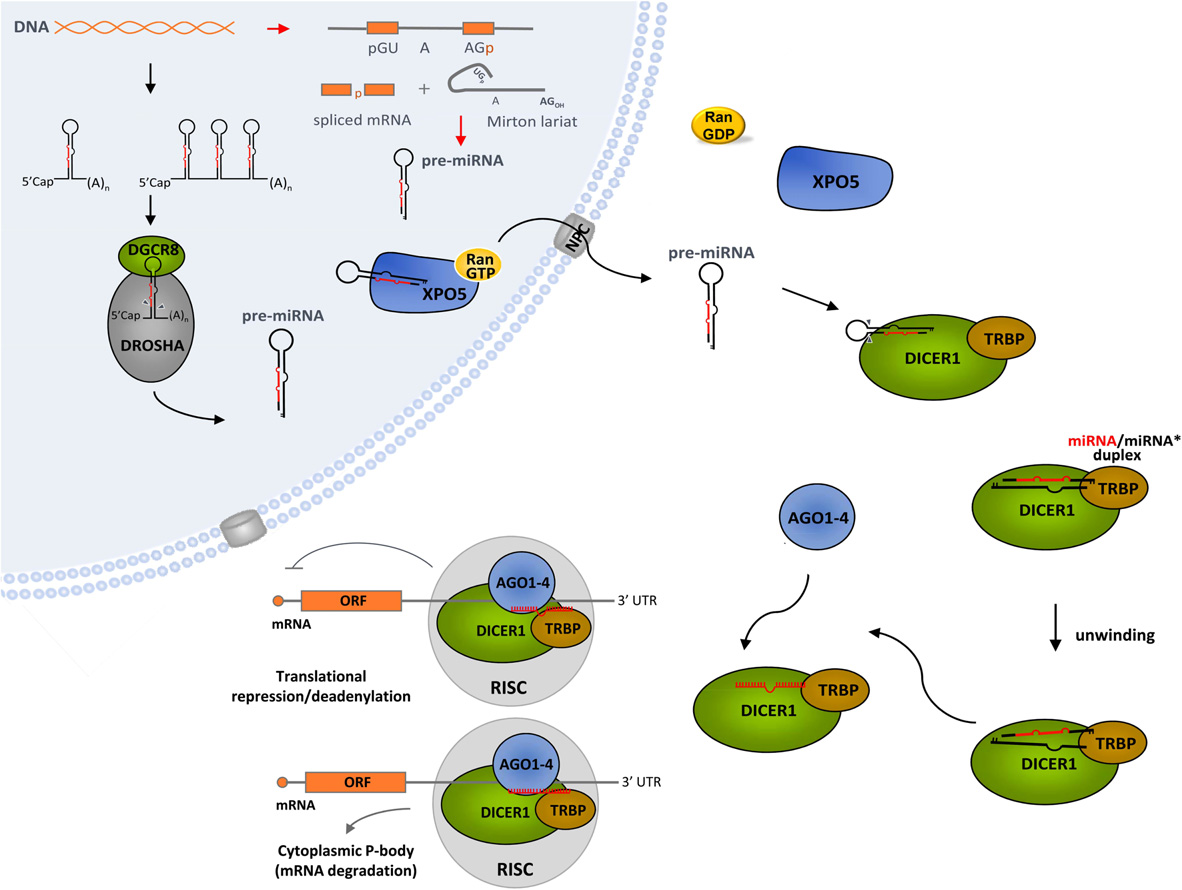
\includegraphics[width=1\linewidth]{figures/miRNA_biogenesis.png}
  \caption{Depiction of the canonical (and mirtron) pathway of microRNA biogenesis
  and microRNA mechanism of action. miRNA biogenesis begins in the nucleus, where
  the pri-miRNA is transcribed, then cut by Drosha to the pre-miRNA and exported
  into the cytoplasm by Exportin 5 (XPO5). Mirtrons do not require Drosha processing.
  The pre-miRNA is then bound by Dicer, which (aided by TRBP) cuts and unwinds the miRNA into
  its mature form. RISC is then formed and, guided by the miRNA, regulates gene expression by translational
  repression or degradation of mRNA. See text for more details.
  Black arrows depict the movement of miRNA molecules through the process, and
  grey arrows the action of RISC on the target mRNA.
  grey arrow 
  ORF: open reading frame (the protein-coding section) of mRNA.
  Figure reprinted with permission from Melo and Esteller \citep{Melo2011}.}
  \label{fig:mirna-biogenesis}
\end{figure}




\subsection{MicroRNA mechanism of action}\label{microrna-mechanism}

RISC is the effector of RNA interference, and Ago functions as its catalytic
engine. MicroRNA sequence guides the RISC to target messenger RNAs
\citep{Filipowicz2008}. Figure \ref{fig:mirna-biogenesis} illustrates a rough
outline of how miRNAs act to regulate mRNA expression.

Target recognition is based on sequence complementarity of the miRNA and mRNA.
In animal miRNAs this complementarity is almost always limited \citep{Ambros2004}.
Nucleotides at positions 2-8 of the 5' end of the microRNA have been found
crucial to target mRNA matching; these nucleotides are termed the miRNA "seed sequence".
miRNA target sequences are mostly located in the 3' UTR (untranslated region)
of the mRNA transcript, but in some instances target sites also reside in the
coding region or 5' UTR of the mRNA \citep{Bartel2009}.

MicroRNAs act through inhibition of mRNA translation or destabilization and
subsequent degradation of mRNA. The exact mechanisms by which the miRNA and
Ago induce translational repression or destabilization of mRNA are unclear
\citep{Filipowicz2008}. Translational inhibition was earlier believed to be
the major form of miRNA action in animals, but recent evidence suggests that
mRNA destabilization predominates \citep{Guo2010}. Rarely, the mRNA can be
directly cleaved by Ago \citep{Du2005}.

mRNAs bound to RISC accumulate in so called processing bodies (P-bodies),
which are known sites of mRNA catabolism and translational repression in the
cytoplasm. The localization in P-bodies, however, appears to be a consequence
of RNA silencing, not the cause, and is reversible \citep{Eulalio2007}.

Interestingly, several alternative mechanisms of action for microRNA have been
reported, illustrating the complexity and diversity of microRNA biology and
gene regulation. For example, some miRNAs can increase the translation of
target mRNA instead of repressing it \citep{Vasudevan2007}, miR-373 was found
to target DNA promoter areas and act to induce gene transcription
\citep{Place2008}, and miR-328 targets a protein to prevent inhibition of mRNA
translation \citep{Eiring2010}.




\subsection{MicroRNA function}\label{microrna-function}

MicroRNAs assert extensive control over the transcriptome, and have been found
to participate in regulation of almost all studied cellular processes,
including embryo development, cell proliferation and differentiation,
apoptosis, and metabolism. More than 60\% of human mRNA transcripts are
predicted to be regulated by miRNAs and most have target sites for several
different miRNAs \citep{Friedman2009}. Furthermore, a single microRNA can have
as many as hundreds or thousands of target mRNAs.

The effect of a single miRNA on the expression of
its target tends to be subtle \citep{Baek2008}. Thus, microRNAs are considered
fine-tuners of gene expression. However, the modest effect can be enhanced by
multiple binding sites and multiple miRNAs acting on the same target, enabling
synergistic interactions \citep{Bartel2009}.

% A recent review concluded that mRNA degradation is the
% predominant form of miRNA action in mammals \citep{Guo2010}.

It should be noted, however, that the functional role and importance of many
miRNA-mRNA interactions are unknown, even for validated interaction pairs.
Uncovering these roles is challenging due to the subtle regulatory effects
miRNAs have and, additionally, because of the complexity and robustness of
many cellular regulatory networks \citep{Bartel2009}. Furthermore,
experimentally validated targets have been recognized for only a fraction of
all known microRNAs. Nonetheless, discovering miRNA targets is a critical step
in understanding their function.




\subsection{Quantification of microRNA expression}

The same methods that are employed for quantifying mRNA expression are generally
also applicable to measuring microRNA expression, and the three principal methods
used are qPCR, microarrays and next-generation sequencing
\citep{Huang2011}. However, as Hunt and colleagues in a recent review point
out, there are several challenges in detecting miRNA expression in particular
\citep{Hunt2015}.

MicroRNAs are very short and typically comprise approximately 0.01\% of RNA
typically extracted from any tissue sample. This implies that
miRNA detection methods must be highly sensitive. Additionally, microRNAs from
the same family can differ by only one base, which in turn requires high
specificity to distinguish between members of the same miRNA family. On the
other hand, variation in miRNA processing can result in slight sequence
variations, or isoforms, of a single miRNA, also known as isomiRs
\citep{Lee2010}. This means high specificity or an incorrect
reference sequence (e.g. that of a weakly-expressed isomiR) used for detection
can cause inaccurate measurements. IsomiRs may also have different functions
resulting from altered target specificity \citep{Chugh2012}.

% The existence of the pri-miRNA, pre-miRNA and mature miRNA molecules provides
% an additional challenge for measurement methods, although differentiation
% between these maturation stages is not necessarily required.

These issues mean that miRNA expression data measured with microarrays are often
quite noisy. Proper filtering and normalization techniques are, therefore,
necessary in analyses of such data. A review of different miRNA microarray
platforms and preprocessing methods has been written by Sah et al \citep{Sah2010}.

Many of these methodological limitations are resolved by next-generation
sequencing (NGS) approaches, which are sensitive and
reliable in quantifying known miRNAs and enables identification of novel ones
\citep{Huang2011}. Sequencing can detect variations of single nucleotides and
does not depend on previously identified sequences. However, not
all identified short RNAs are functional miRNAs, and NGS conveys its own set
of problems relating to significant computational complexity and
validation efforts to distinguish relevant data from noise
\citep{Hunt2015}.
